\documentclass[a4paper]{article}
\usepackage{graphicx}
\usepackage{amssymb}
\usepackage{amstext}
\usepackage{amsmath}
\usepackage[brazilian]{babel}
\usepackage[utf8]{inputenc}
\usepackage[T1]{fontenc}
\usepackage{listings}

\usepackage[brazilian]{babel}
\usepackage[utf8]{inputenc}
\usepackage[T1]{fontenc}

\usepackage{listings}
\usepackage{color}

\graphicspath{ {/home/daemonio/} }

\definecolor{dkgreen}{rgb}{0,0.6,0}
\definecolor{gray}{rgb}{0.5,0.5,0.5}
\definecolor{mauve}{rgb}{0.58,0,0.82}

\lstset{frame=tb,
  language=Python,
  aboveskip=3mm,
  belowskip=3mm,
  showstringspaces=false,
  columns=flexible,
  basicstyle={\small\ttfamily},
  numbers=none,
  numberstyle=\tiny\color{gray},
  keywordstyle=\color{blue},
  commentstyle=\color{dkgreen},
  stringstyle=\color{mauve},
  breaklines=true,
  breakatwhitespace=true,
  tabsize=3
}

\begin{document}

\title{%
  Distribuição e Execução de Tarefas com pagamento em moedas IOTA \\
  \large Blockchains, Criptomoedas e Outras Aplicações}
    
\author{
  Ferreira, Marcos P.\\
  \texttt{marcospferreira@dcc.ufmg.br}
  \and
  Vieira, Christian \\
  \texttt{chrdcv@gmail.com}
}

\maketitle

\begin{abstract}
Nesse trabalho desenvolveremos um sistema de processamento de tarefas remoto em que clientes pagam o servidor
de execução em IOTA por programa executado. A comunicação entre cliente e servidor é através do tangle, assim
retirando a necessidade de um conhecer o IP do outro. Após a execução da tarefa, o cliente realiza um pagamento
em moedas IOTA para receber a saída de sua tarefa.
\end{abstract}

\section{Introdução}\label{sec:Introduction}

Toda criptomeda requer três componentes: um protocolo de consenso, uma ``ledger'' distribuída e um contrato inteligente.
Para o bitcoin, os componentes correspondentes são: proof of work, blockchain e as transações. No caso da Ethereum, as
componentes são proof of work (e, futuramente, proof of stake), blockchain e scripts em solidity. Porém, nem toda criptomoeda
usa a estrutura de blockchain.

A IOTA revoluciona o sistema acima ao abandonar a blockchain e usar uma nova estrutura de dados: o tangle, um grafo acílico
e direcionado em que nenhuma estrutura de encadeamento (ou chain) é necessária. Cada transação é um nodo nesse grafo e de
cada nodo saem duas arestas ligando em duas outras transações. As arestas indicam que aquele nodo verificou o proof of work
dos nodos ligantes. Novas transações chegam, e novas ligações serão feitas para verificar as transações existentes, e quando
um determinado nodo é visto por todas as novas transações, isso é, existe um caminho de toda nova transação para este
nodo, então ele é validado no tangle.

Há várias vantagens desse sistema. Primeiro que não é necessário mineradores já que cada nova transação precisa verificar
duas já existentes. Outra vantagem é a possibilidade de se enviar transações de valor zero, pois mesmo ela não acrescentando
``valor`` na rede, ela ajudou no consenso validando duas outras transações.

Usaremos nesse trabalho o tangle e também transações IOTA para elaborar um serviço cliente-servidor de execução de tarefas
em que toda comunicação é realizada pelo tangle, como também o pagamento da tarefa do cliente para o servidor. A vantagem dessa
abordagem é que o cliente não precisa saber o endereço IP do servidor, pois toda a comunicação é feita via tangle.

\section{Objetivos}\label{sec:Goals}

O objetivo é mostrar a eficiência e flexibilidade da moeda IOTA como meio de pagamento de serviços em uma economia
machine-to-machine. Será desenvolvido uma pequena plataforma cliente-servidor em que clientes enviam tarefas a serem
executadas por um servidor e o custo do processamento é pago via criptomoeda IOTA. Esse tipo de sistema é conhecido
como Processamento em Batch, e tem a característica de que tarefas no mesmo batch são executadas sequencialmente e que
elas não são iterativas.

Forneceremos como funcionará a comunicação e como o servidor gerencia clientes em conjunto
com as transações envolvendo a criptomoeda. Também elaboraremos um simples método para se calcular o custo total
do uso dos recursos do servidor, que se baseia no tempo total de uso dos recursos do servidor.

Por fim, esperamos mostrar que negociações sobre algum serviço entre dispositivos já é realidade e o pagamento pode ser feito
por moedas digitais, como a IOTA.

\section{MyIOTA: API IOTA}

Para realizar transações em criptomoeda é necessário o uso de uma API. Nesse trabalho, utilizamos a API Pyota, que fornece um conjunto
de funções para gerenciar transações IOTA. Criamos também uma API baseado na primeira, chamada de MyIOTA. Ela é uma simples classe
que fornece métodos como ``send\_transfer()'' e ``get\_balance()'' para facilitar a programação. Além disso, ela fornece segurança
nas transações IOTA, garantindo que nenhum endereço de envio será reusado.

Abaixo exemplos comuns da API. Basta seguir passos pré-definidos para enviar e receber IOTAS sem complicações.

\subsection{Enviar IOTAS}
Para exemplificar, a seguir um script para enviar 100 IOTAS para o endereço: UXIKP...VVDQD.

\begin{lstlisting}
from wallet import MyIOTA

# Set your SEED.
SEED = 'G9OJZJ...EWTEB'

# Let's create our connection.
iota = MyIOTA('http://localhost:14265', SEED)

# Init the wallet
iota.init_wallet()

# Create 10 addresses
if iota.is_empty_wallet():
    iota.make_addr_list(start_index = 0, n = 10)

# Get fund for the 10 addresses.
print 'Your total fund is: ', iota.get_total_fund()

# Destination addr
addr = 'UXIKP...VVDQD'
dest_addr = iota.Address(addr)

# Get inputs and change_addr
inputs, change_addr = iota.get_inputs(transfer_value)

# Outputs
output1 = iota.prepare_transfer(transfer_value, \
          dest_addr, tag = 'TEST', msg = 'HELLO')

transfer_value = 100

# Send
iota.send_transfer(transfer_value, inputs, \
     outputs, change_addr)
\end{lstlisting}

\subsection{Receber IOTAS}

Para ``receber'' suas IOTAS, isso é, verificar no tangle o seu saldo total, basta executar ``find\_ transactions()'' e
verificar se as transações foram confirmadas na rede.

\begin{lstlisting}
#!/usr/bin/env python2.7

from wallet import MyIOTA

# Set your SEED.
SEED   = 'WXBTI...ARINL'

# Let's create our connection.
iota = MyIOTA('http://localhost:14265', SEED)

iota.init_wallet()

iota.make_addr_list(start_index = 0, n = 10)

print 'Your total fund is: ', iota.get_total_fund()

txn_list = iota.find_transactions()

for txn in iota.get_info_transactions(txn_list):
    confirmed_t, addr_t, value_t, tag_t, msg_t = txn

    if confirmed_t:
        print addr_t, value_t
\end{lstlisting}

Outras funções foram implementadas na MyIOTA. Para ter acesso completo a API, veja: XXXX.

\section{Metodologia}\label{sec:Metodology}

\subsection{Visão Geral}

A moeda IOTA utiliza o Tangle como Ledger e que funciona bem diferente da Blockchain, adotada por muitas criptomoedas. Essa construção
permite o uso de transações de valor zero, onde o custo seria simplesmente aprovar duas outras transações. Nesse trabalho, iremos
lidar com o modelo cliente-servidor, onde o cliente envia um programa para o servidor executar e depois ele paga para receber
o resultado.

\begin{figure}[!htb]
\centering
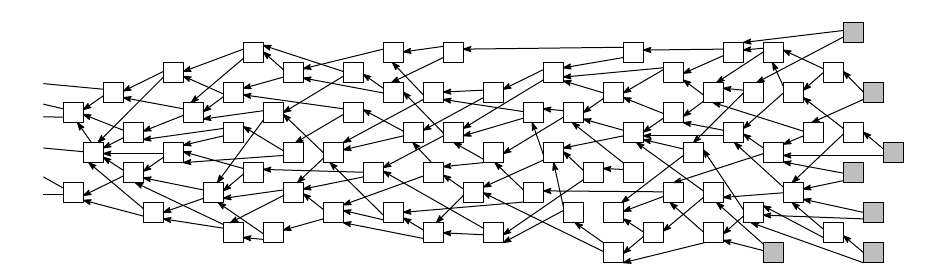
\includegraphics[scale=0.4]{tangle.jpg}
\caption{IOTA Tangle}
\label{fig:tangle}
\end{figure}

A gerência da carteira IOTA será feita por uma API própria (MyIOTA), que foi desenvolvida para esse trabalho, e que, por sua vez, foi
desenvolvida usando a API Python chamada PyOta.

\begin{enumerate}
\item Cliente conecta o servidor por algum endereço IOTA disponível.
\item Cliente realiza transações-zero onde o campo ``message'' contém o programa a ser executado.
\item Servidor procura no Tangle transações que envolvem seu endereço.
\item Servidor detecta transações novas, as recebe e considera o campo mensagem como o script da tarefa.
\item Servidor executa o programa.
\item Servidor envia para o Cliente o preço $p*t$ e um novo endereço IOTA para pagamento.
\item Cliente realiza o pagamento em IOTA.
\item Servidor valida o pagamento.
\item Servidor retorna a saída do programa do cliente (arquivo de saída).
\end{enumerate}

Podemos ver que a comunicação entre cliente e servidor é exclusivamente via Tangle. Através de transações de valor zero, o cliente
envia como mensagem o corpo do programa a ser executado. O servidor consegue recuperar as transações que usam seu endereço, como
também o corpo da mensagem, onde está a tarefa a ser executada.

Outro detalhe é que o servidor executa a tarefa primeiro porque ele precisa do tempo total para retornar o preço do serviço.

\subsection{Test Net}

Utilizamos uma rede teste IOTA disponibilizada no site XXX. Para facilitar, criamos containers dockers para executar uma test
net com um só comando. O link do Docker pode ser visto em YYY.

\subsection{Configuração do servidor}

O servidor monitora o tangle, isso é, ele executa uma chamada a ``get\_ transactions(addr)'' que retorna todos as transações destinadas
ao endereço passado. O servidor mantém uma lista para saber quais transações já foram lidas e quais são novas. Uma tarefa pode ser enviada
usando várias transações, logo o servidor também sabe se todo o conteúdo de uma tarefa já foi lido do tangle. Novas tarefas são checadas a cada
5 minutos no tangle, um tempo aparentemente bom para tanto evitar o custo de constantemente verificar o tangle quanto para não demorar receber novas tarefas.

O preço total é calculado pela fórmula: \fbox{$\text{preco} = p * t$}. Onde $t$ é o tempo total e $p$ é o preço de meia-MIOTA, ou $500.000$ iotas.
Atualmente, na escrita desse trabalho, uma MIOTA é $\text{US }1.80$, então $p = \text{US }0.9$.

Por enquanto o servidor não possui restrição quanto ao número de tarefas. Aparentemente, ele pode executar toda e qualquer tarefa que chegar.

O comportamento geral do servidor é:

\begin{enumerate}
\item Servidor checa o tangle.
\item Servidor obtém tarefas. Confere se já existe ou tarefa nova.
\item Servidor executa tarefas.
\item Servidor envia transação-zero para o cliente com a tag ``TASK \_ID|SERV \_RESPONSE'' ...
\item ... e no corpo da mensagem o valor da tarefa + o endereço.
\item Servidor espera pagamento no endereço dado.
\item Servidor envia saida da tarefa para o cliente via transação-zero.
\end{enumerate}

\subsection{Configuração do cliente}

O cliente pode ser qualquer dispositivo que necessite executar alguma tarefa: celulares, notebooks, tablets, sensores, etc.
Esse trabalho funciona de forma semelhante a serviços na nuvem: um cliente aloca recursos, como máquinas virtuais, e no fim
paga pelo o uso.

O cliente escolhe a tarefa a ser executada, como um script python, por exemplo. O próximo passo é encapsular esse arquivo dentro
do corpo de uma transação zero. Para isso foi criado um módulo chamado ``MAM.py'' que recebe um arquivo como entrada e retorna
transações IOTA, após isso, o cliente repassa essas transações para a rede. O cliente também passa no corpo da mensagem o
seu endereço para que o servidor se comunique com ele.

Quando a tarefa termina no lado do servidor, o servidor de posse do endereço do cliente enviado no corpo da mensagem, envia uma
transação-zero para o cliente sendo o corpo da mensagem o valor em IOTAS a ser pago e o endereço de pagamento. O cliente, por sua vez,
ao acessar o tangle, verificará a transação enviada pelo servidor e pagará o valor no endereço especificado.

Quando o servidor receber o pagamento (transação confirmada), ele envia a saída da tarefa para o cliente.

O comportamento geral do cliente é:

\begin{enumerate}
\item Cliente envia tarefa para servidor via transação-zero ...
\item ... e envia também seu endereço de comunicação.
\item Cliente espera resposta do servidor no endereço dado.
\item Cliente recebe resposta do servidor com valor da tarefa  + endereço.
\item Cliente envia uma transação de valor para servidor.
\item Cliente espera resposta do servidor com a saída da tarefa.
\end{enumerate}

\section{Resultados}\label{sec:Output}

O resultado foi como esperado. O cliente enviou tranzações-zero com a tarefa como mensagem e o servidor conseguiu recuperá-las.

Abaixo um pequeno transcript do ocorrido. Todos os arquivos podem ser obtidos em xXXXXX.

\subsection{Cliente: Envio de tarefa}

O cliente deseja enviar a seguinte tarefa:

essa tarefa fatora um determinado número inteiro. O arquivo é ``test.py''. O cliente envia a tarefa:

\begin{lstlisting}[language=bash]
  $ ./client.sy test.py endereco
\end{lstlisting}

O script segura o terminal, pois ele checa o tangle a cada 5 minutos por uma resposta do servidor. Quando o servidor responde,
o cliente mostra o valor da execução da tarefa e o endereço que receberá o pagamento.

O cliente, em seguida, realiza o pagamento.

\subsection{Problemas Encontrados}

O maior problema encontrado foi que a ``test net'' da IOTA não valida as transações automaticamente. Se comparado com a Ethereum onde a test net
contém um ``minerador'' falso que valida as transações de teste, a testnet da IOTA deixa a desejar. O problema ocorre que quando
realizamos uma transação, ele não é confirmada, então é impossível utilizar a mesma SEED para realizar transferências. O que foi feito,
como teste, foi selecionar uma nova SEED toda vez que uma transação de valor precisou ser feita. Isso resolveu o problema da nulidade
da carteira, mas não o problema de transações pendente.

Porém, mesmo em modo pendente, as transações eram válidas e possivelmente poderiam fazer parte da rede principal da IOTA
sem problemas.

\section{Futuras melhorias}\label{sec:Future}

Uma lista de futuras melhorias para o sistema.

\begin{enumerate}
\item Testar na main net só para verificar o desempenho e corretude.
\item Verificar condições de corrida já que vários clientes são atendidos ao mesmo tempo.
\item Fornecer melhores recursos para as tarefas, como banco de dados, containers, virtualização, etc.
\item Verificação de segurança. Como está implementado, um atacante pode alterar tarefas de clientes legítimos.
\end{enumerate}

\section{Conclusão}
O objetivo do trablhao foi aplicar a tecnologia da moeda IOTA em um serviço de execução de tarefas. A tecnologia nos permitiu uma
comunicação descentralizada entre cliente e servidor, e também a propria transação financeira para pagar o serviço. O objetivo do
trabalho foi alcançado através da execução de scripts exemplos mostrando o funcionamento do sistema. Foi criada uma API própria,
chamada de MyIOTA, que funciona como uma carteira, e com funções de enviar e receber transações.

O sistema pode ainda melhorar principalmente no aspecto de segurança, porém, como prova de conceito, ele está bastante funcional.

%\bibliographystyle{unsrt}
%\bibliography{my_references}
\end{document}

\section{Referências}
https://currencio.co/miota/usd/
https://github.com/daemonio/docker-iota-testnet